\section{Eclipse Modeling}
\href{http://eclipse.org/modeling/emf/}{The Eclipse Modeling Framework}
is a tool for designing and manipulating models in Eclipse with many
facilities for code generation and persistent data manipulation. It is
important to be familiar with this framework in order to understand this
project. The most important features used are:
\begin{enumerate}
    \item \href{www.eclipse.org/ecoretools/}{\textbf{Ecore tools}} : A graphical meta-model editor
    \item \href{https://wiki.eclipse.org/OCL/OCLinEcore}{\textbf{OCLinEcore}} : A modified version of the \href{http://www.eclipse.org/modeling/mdt/?project=ocl}{Object Constraint Language} used to define structural constraints for an instance of a meta-model
    \item \textbf{Code Generation} : A large part of the code in the plug-in was generated by Ecore. 
    \item \href{http://www.eclipse.org/sirius/}{\textbf{Sirius}} : A framework for creating graphical DSLs based on Ecore models
\end{enumerate}
These tools are Eclipse plug-ins which must be installed first before
modifying the plugin. If you installed the version of Eclipsed used for modeling,
you will find a button in the toolbar like in figure \ref{fig:plugin_button}.
\begin{figure}[H]
    \centering
    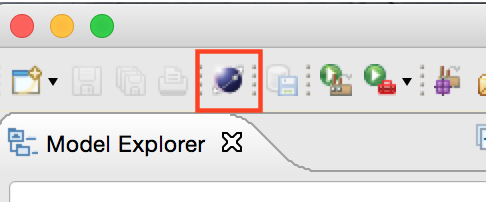
\includegraphics[width=0.3\textwidth]{modeling_button}
    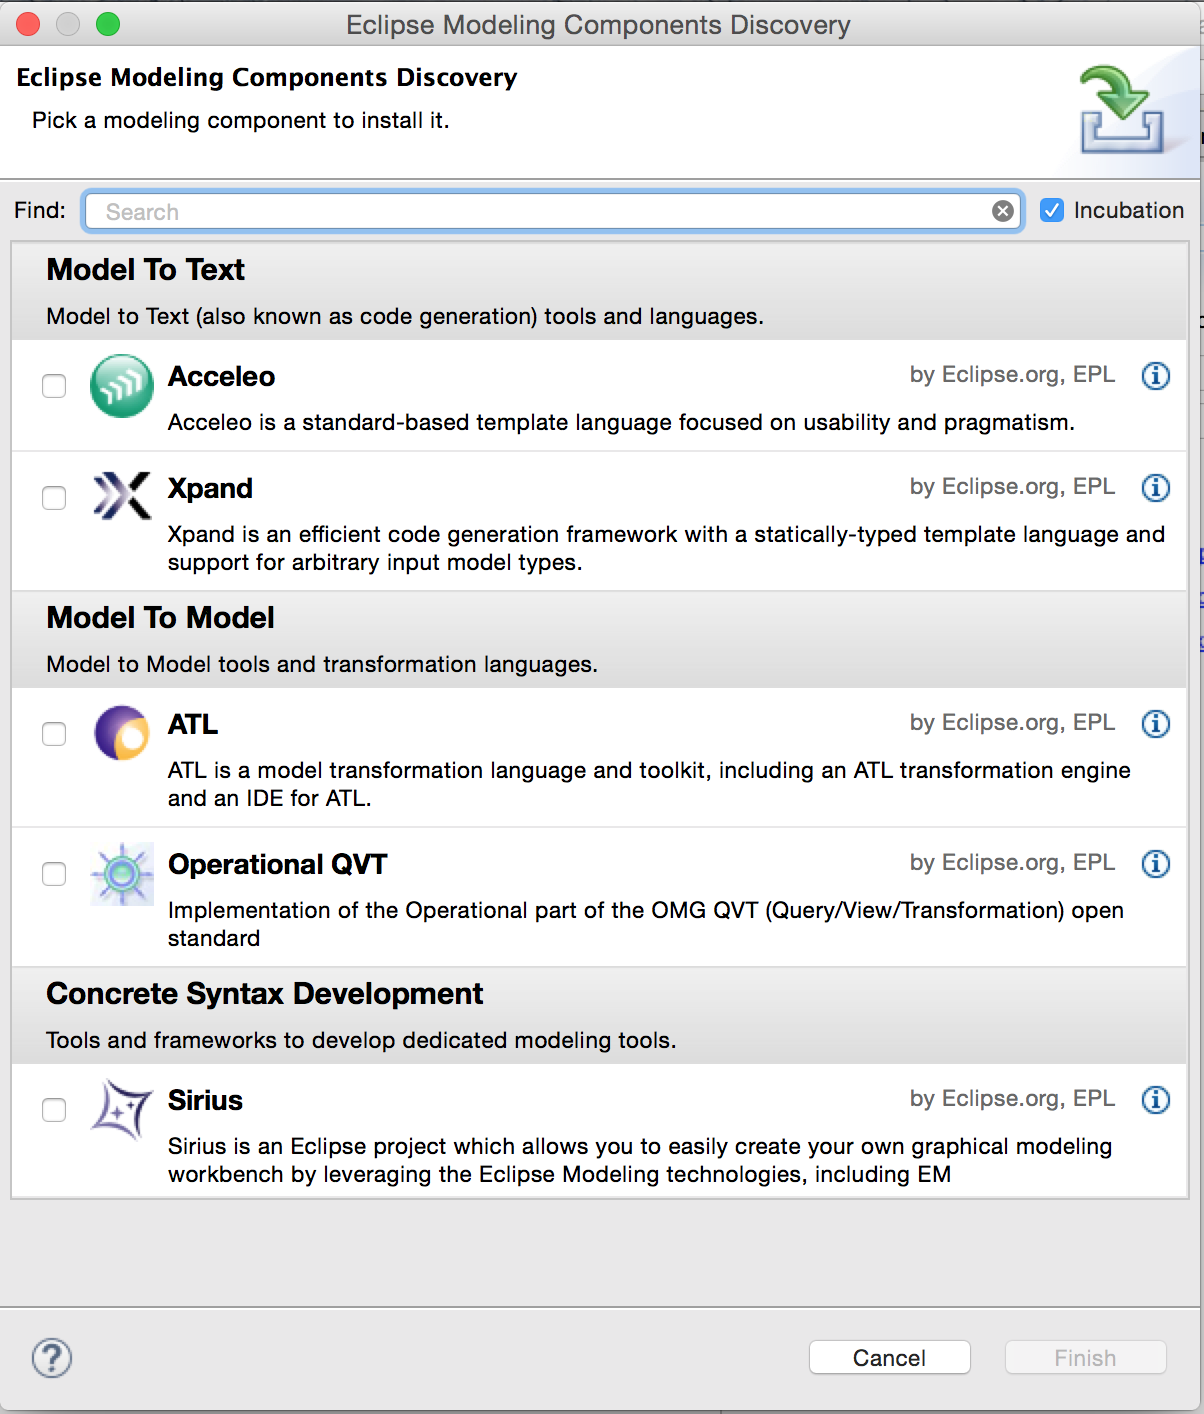
\includegraphics[width=0.3\textwidth]{plugin_selection}
    \caption{Install modeling plugins}
    \label{fig:plugin_button}
\end{figure}
This opens a window with many modeling plugins to install, you should install
Sirius and EcoreTools. 
